\section{Mid-Training: Premium-Data Annealing and the Context Gate}\label{sec:midtrain}

Mid-training -- the interval between the main pretraining run and post-training -- offered two candidate interventions for the 596M base: extending the context window, and annealing onto premium data during a learning-rate cooldown \citep{hu2024minicpm, olmo20242}. The first was killed by a cheap diagnostic before any budget was spent; the second is the one stage in this study that reaches a \emph{win} under the per-stage eval-completeness gate. Table~\ref{tab:midtrain} summarizes the stage.

% tab_midtrain.tex -- mid-training anneal (premium mix) vs iso-token FineWeb control vs un-annealed base.
% Sources: verdict.json (corpora, short_ctx_non_regression, ecl_ladder), c5_evidence.json in
%   Qwen3-0.6B/experiments/2026-06-30_qwen3-0.6b_midtrain-anneal/
%   step0 gate: Qwen3-0.6B/experiments/2026-06-27_qwen3-0.6b_midtraining/step0_diagnostic.json
\begin{table}[t]
\centering
\caption{Mid-training anneal at 596M: premium-mix anneal vs.\ an iso-token FineWeb-Edu control vs.\ the un-annealed base.
Both arms run the identical 1-sqrt cooldown (peak LR $2.5\times10^{-4} \rightarrow 2.5\times10^{-5}$, 10\% floor) for 2{,}300 steps $\times$ 65{,}536 tokens $=$ 150.7M tokens per cell ($\approx$13\% of the 1.19B-token pretrain), $n{=}3$ seeds per arm; only the data differs (iso-FLOP by construction).
Top block: BPB per corpus, with the anneal$-$control improvement and its paired across-seed 95\% CI (suite \texttt{text-lm-v2}).
The control barely moves off the base ($+0.0050$ code, $+0.0036$ wikitext-2 BPB), i.e.\ LR decay plus 150M extra FineWeb tokens alone do approximately nothing --- the data, not the schedule, carries the effect.
The wikitext-2 gain is small but significant, violating the pre-registered expected null on English; it is reported as-is.
Bottom block: effective-context-length passkey ladder (suite \texttt{ecl-ladder-v1}, $n{=}40$ probes per rung per cell, arms pooled over 3 seeds, Wilson 95\% CIs); the base's anomalous 4096-rung accuracy (exactly 0.025) is repaired to 0.400 by both arms, and no cell regresses vs.\ base at any rung.
A separate step-0 diagnostic (\texttt{step0\_diagnostic.json}) had gated context \emph{extension} to propose-only: the base scores 0.083 at its own 4096-token trained window (threshold 0.5, gate FAIL).
Source files: \texttt{verdict.json}, \texttt{c5\_evidence.json} (2026-06-30 midtrain-anneal), \texttt{step0\_diagnostic.json} (2026-06-27 midtraining).}
\label{tab:midtrain}
\footnotesize
\setlength{\tabcolsep}{3.5pt}
\begin{tabular}{lcccc}
\toprule
 & Base & Control (FineWeb) & Anneal (mix) & Anneal $-$ Control (95\% CI) \\
\midrule
\multicolumn{5}{l}{\emph{BPB (lower is better; improvements are positive), suite \texttt{text-lm-v2}}} \\
Code (Python) BPB        & 2.1286 & 2.1236 & 1.8520 & $+0.2716$ $[+0.2641,\,+0.2792]$ sig.\ \\
wikitext-2 BPB           & 1.2256 & 1.2220 & 1.2062 & $+0.0157$ $[+0.0140,\,+0.0174]$ sig.\ \\
$\Delta$ vs.\ base, code       & --- & $+0.0050$ & $+0.2766$ & \\
$\Delta$ vs.\ base, wikitext-2 & --- & $+0.0036$ & $+0.0194$ & \\
\midrule
\multicolumn{5}{l}{\emph{Passkey accuracy by context rung (suite \texttt{ecl-ladder-v1}; Wilson 95\% CI; arms pooled, $3{\times}40$ probes)}} \\
512-token rung  & 0.200 $[0.105,\,0.348]$ & 0.308 $[0.233,\,0.396]$ & 0.817 $[0.738,\,0.876]$ & \\
4096-token rung & 0.025 $[0.004,\,0.129]$ & 0.400 $[0.317,\,0.489]$ & 0.400 $[0.317,\,0.489]$ & \\
\bottomrule
\end{tabular}
\end{table}


\subsection{The step-0 diagnostic that gated off context extension}\label{sec:midtrain-gate}

Before budgeting a context-extension run, a step-0 passkey-retrieval diagnostic \citep{mohtashami2023landmark} probed the base checkpoint at and beyond its trained window. The pre-registered gate required accuracy $\geq 0.5$ at the trained length of 4096 tokens; the base scored 0.083 (Table~\ref{tab:midtrain}). Per-length accuracies were 0.333 at 512, 1024, and 2048 tokens, 0.083 at 4096, 0.583 at 6144, and 0.250 at 8192. The diagnostic nominally reports an effective context length of 6144 because the 6144-token rung happens to clear the absolute threshold, but the ladder is non-monotone and the above-trained-window spike at 6144 is better read as instability of a small unstamped probe than as genuine capability; the decision variable is the trained-length accuracy, and it failed by a factor of six. The recorded verdict is that context extension is moot -- the base collapses \emph{before} its trained window -- so the extension sub-stage stayed propose-only and no extension run was launched. This is the pattern that effective-context benchmarks document at much larger scales, where usable context falls well short of the nominal window \citep{hsieh2024ruler}; here the gap is severe enough at 596M and 1.19B training tokens that extending the nominal window would optimize the wrong margin.

\subsection{Annealing onto the premium mix under an iso-token control}\label{sec:midtrain-anneal}

The anneal starts from the faithful base checkpoint (1.19B FineWeb-Edu tokens \citep{penedo2024fineweb}) and runs a ``1-sqrt'' cooldown from peak learning rate $2.5\times10^{-4}$ to $2.5\times10^{-5}$ (a 10\% floor, 46 warmup steps) for 2{,}300 steps $\times$ 65{,}536 tokens $=$ 150.7M tokens per cell, $\approx$13\% of the pretraining budget, with $n{=}3$ seeds per arm. The treatment anneals onto the 50/50 dclm-edu/FineWeb-Edu mix selected by the data-composition study \citep{li2024datacomp} (Table~\ref{tab:data}); the control runs the identical cooldown on iso-token FineWeb-Edu. Exactly one variable (the data) differs, so the comparison is iso-FLOP by construction, and the design eats the standard confound of anneal experiments: whatever the learning-rate decay plus 150M additional tokens do on their own is captured by the control.

The answer is that they do approximately nothing. The control moved $+0.0050$ BPB on code and $+0.0036$ BPB on wikitext-2 relative to the un-annealed base (text-lm-v2; Table~\ref{tab:midtrain}), while the mix anneal beat the control on code by $+0.2716$ BPB (95\% CI $[+0.2641, +0.2792]$, 3 seeds, paired), significant (text-lm-v2; Figure~\ref{fig:data-anneal}). The data, not the schedule, carries the effect. Against the constant-learning-rate continued-train sibling on the same mix ($+0.5904$ BPB on code, 95\% CI $[+0.5532, +0.6277]$; an upper-bound reference at a similar 131M-token budget, not an iso-FLOP comparison), the 150.7M-token cooldown retains $\approx$46\% of the effect.

On English, the pre-registration expected an honest null; the measurement violated it: wikitext-2 improved by $+0.0157$ BPB (95\% CI $[+0.0140, +0.0174]$, 3 seeds, paired), significant (text-lm-v2), $\approx$1.3\% relative. This is reported as an exploratory violation of the pre-registered expectation, not as a claim: the point estimate is the same size as the constant-learning-rate sibling's $+0.0161$ BPB, which was \emph{not} significant, and what pushed the anneal's identical-size effect past significance is the cooldown's much tighter across-seed spread. A same-size estimate flipping significance purely through variance is exactly the situation pre-registration exists to flag.

\begin{figure}[t]
\centering
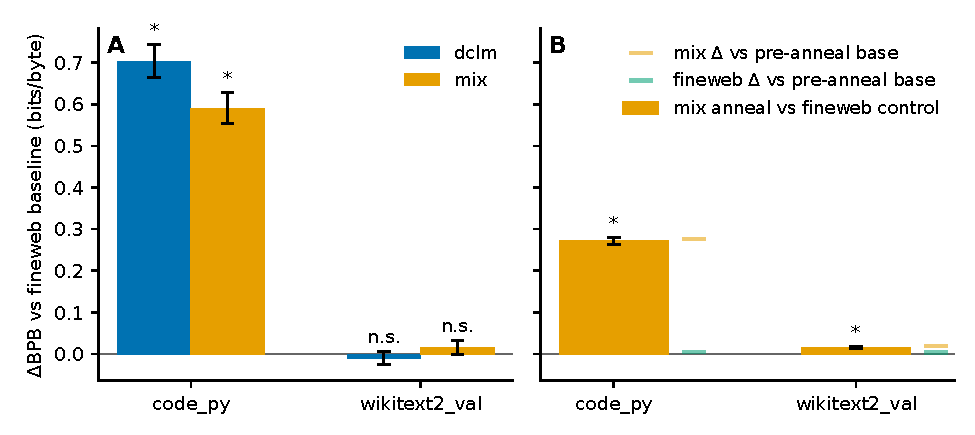
\includegraphics[width=\linewidth]{figures/fig_data_anneal}
\caption{Data-composition and mid-training-anneal effects: BPB improvement over the FineWeb-Edu control (positive is better) with paired across-seed 95\% CIs, $n{=}3$ seeds per arm, suite \texttt{text-lm-v2}, on \texttt{code\_py} and wikitext-2. Data-composition arms (dclm-edu; 50/50 mix) train 2{,}000 steps $\times$ 65{,}536 $=$ 131.1M tokens per cell at full LR; the mid-training anneal arms run the 1-sqrt cooldown for 2{,}300 steps $\times$ 65{,}536 $=$ 150.7M tokens per cell ($\approx$13\% of the 1.19B-token pretrain) against an iso-token FineWeb-Edu control. Sources: \texttt{verdict.json} of the 2026-06-24 dclm-vs-fineweb, 2026-06-26 data-mix-composition, and 2026-06-30 midtrain-anneal experiments; rendered by \texttt{fig\_data\_anneal.py}.}
\label{fig:data-anneal}
\end{figure}

\subsection{The effective-context-length ladder}\label{sec:midtrain-ecl}

Both anneal arms and the base were then scored on a passkey ladder over context rungs 512--8192 (ecl-ladder-v1; $n{=}40$ probes per rung per cell, arms pooled over 3 seeds, Wilson 95\% CIs; Figure~\ref{fig:ecl-ladder}). The base exhibits an anomalous dip at its own trained length: 4096-rung accuracy is exactly 0.025, far below its 512-rung 0.200. Both anneal arms repair the dip to 0.400 -- the FineWeb-Edu control included, so the repair does not require the premium data. The mix arm additionally lifts the pooled 512-token rung to 0.8167 versus 0.20 for the base, and no cell regresses relative to the base at any rung (the recorded regression list is empty). The mechanism of the trained-length dip, and of its repair by an ordinary cooldown, is unexplained; with $n{=}40$ probes per rung the ladder characterizes the phenomenon without diagnosing it, and it is flagged as an open question in Section~\ref{sec:limitations}. The step-0 diagnostic's independent 4096-token failure (0.083) is consistent with the same anomaly.

\begin{figure}[t]
\centering
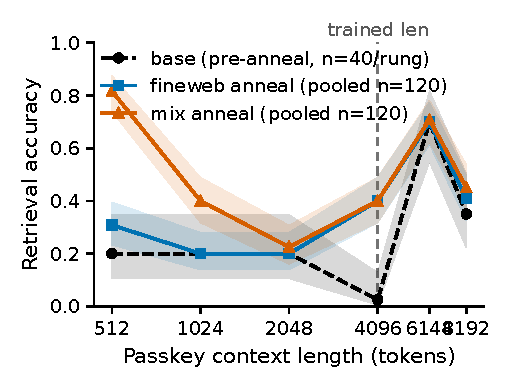
\includegraphics[width=\linewidth]{figures/fig_ecl_ladder}
\caption{Effective-context-length passkey ladder (suite \texttt{ecl-ladder-v1}): accuracy by context rung (512--8192 tokens) for the un-annealed base, the FineWeb-Edu-anneal control, and the mix-anneal treatment. $n{=}40$ probes per rung per cell; anneal arms pooled over 3 seeds ($3\times40$ probes per point); Wilson 95\% CIs. Both anneal arms (150.7M tokens per cell, identical cooldown) repair the base's anomalous 4096-rung dip ($0.025 \rightarrow 0.400$), and no cell regresses versus the base at any rung. Sources: \texttt{ecl\_ladder.json} and \texttt{verdict.json} (2026-06-30 midtrain-anneal); rendered by \texttt{fig\_ecl\_ladder.py}.}
\label{fig:ecl-ladder}
\end{figure}

\subsection{Robustness and the stage verdict}\label{sec:midtrain-verdict}

Two integrity checks qualify the headline. First, one treatment cell (mix, seed 0) was twice terminated by an external SIGTERM (exit code 143; not the resource watchdog, whose kill line was never approached) and resumed; the resume rebuilds the data shuffle without fast-forwarding, which if anything disadvantages the treatment. Excluding that cell entirely, the code effect holds: $+0.2717$ BPB (95\% CI $[+0.2333, +0.3100]$), significant, with the caveat that the treatment arm drops to $n{=}2$ seeds and the CI widens accordingly; the excluded cell's BPB (1.8521) is not a within-arm outlier (arm range 1.8489--1.8550). Second, the loaded token pools differ by $\approx$0.7\% in the control's favor, and the control lost anyway -- the imbalance is conservative with respect to the conclusion.

Under the per-stage eval-completeness gate, mid-training required three hard items -- the effective-context-length ladder, short-context non-regression, and the anneal gain against an iso-token control -- and all three are present, with the single-variable iso-FLOP check recorded in the run ledger. Mid-training is therefore the one lifecycle stage in this study that is hard-complete under the gate, and its recorded verdict is \emph{win}.
